\subsubsection{Shorter Paths}
\label{sec:sphinx:shorterpaths}

\textit{under construction} TODO: add reference to paper

SPHINX packets define a maximum packet length $r$\footnote{HOPR nodes use by default a path length of three and refuse the processing of packets with greater path lengths.}, meaning $r$ intermediate mix nodes and one destination. They also allow the usage of shorter paths of length $v$ with $0 \le v < r$. Despite these packets have the same size and are due to their construction indistinguishable from packet with maximum path length, it not advisable to shorter paths since they introduce observable patterns that deviate from normal usage. By observing these patterns, an adversary can be able to reconstruct route of distinguished packets.

Creating a header for shorter paths require less space, hence in the end of $\beta$, there is free space left, which is filled with \textit{random} data.

\begin{figure}[H]
    \centering
    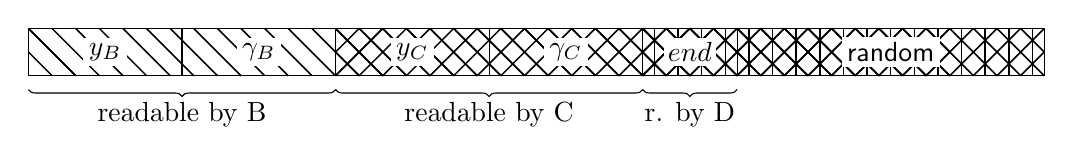
\begin{tikzpicture}
        \def\one{0.6}
        \def\scale{0.9}
        \def\nodeWidth{1.95}
        \def\endWidth{1.2}
        \def\width{3*2*\nodeWidth+\endWidth}
        \foreach \i\name in{0/B,1/C,2/D,3/Z} {
                \begin{scope}[shift={(\i*\nodeWidth*2,0)}]
                    \ifnum\i=0
                        \def\a{11.7}
                        \def\diff{11.1}
                    \fi

                    \ifnum\i=1
                        \def\a{7.8}
                        \def\diff{7.2}
                    \fi

                    \ifnum\i=2
                        \def\a{5.1}
                        \def\diff{4.5}
                    \fi

                    \def\b{\one}
                    \def\lw{0.2}

                    \ifnum\i<3
                        \foreach \x [count=\i] in{0,0.3,0.6,...,\b}{
                                \draw [line width=\lw mm](\x,0)--(0,\x) (\a-\b+\x,\b)--(\a,\x);
                            }
                        \foreach \x [count=\i] in{0,0.3,0.6,...,\diff}{
                                \draw [line width=\lw mm](\x+\b,0)--(\x,\b);
                            }

                        \ifnum\i>0
                            \foreach \x [count=\i] in{0,0.3,0.6,...,\b}{
                                    \draw [line width=\lw mm](0,\x)--(\b-\x,\b) (\a-\b+\x,0)--(\a,\b-\x);
                                }
                            \foreach \x [count=\i] in{0,0.3,0.6,...,\diff}{
                                    \draw [line width=\lw mm](\x,0)--(\b+\x,\b);
                                }
                        \fi

                        \ifnum\i>1
                            \foreach \x [count=\i] in{0.15,0.45,...,\a}{
                                    \draw [line width=\lw mm](\x,0)--(\x,\b);
                                }
                        \fi
                    \fi
                \end{scope}
                \ifnum\i=3
                    \draw (\i*2*\nodeWidth-2*\nodeWidth+\endWidth,0) rectangle (\i*2*\nodeWidth+\endWidth,\one) node [midway,fill=white,inner sep=2pt] {\textsf{random}};
                \else
                    \ifnum\i<2
                        \draw [color=white] (\i*2*\nodeWidth,0) rectangle (\i*2*\nodeWidth+\nodeWidth,\one) node [midway,color=black,fill=white,inner sep=2pt] {$y_{\name}$};
                        \draw (\i*2*\nodeWidth,0) -- (\i*2*\nodeWidth,\one);
                        \draw [color=white] (\i*2*\nodeWidth+\nodeWidth,0) rectangle (\i*2*\nodeWidth+2*\nodeWidth,\one) node [midway,color=black,fill=white,inner sep=2pt] {$\gamma_{\name}$};
                        \draw (\i*2*\nodeWidth+\nodeWidth,0) -- (\i*2*\nodeWidth+\nodeWidth,\one);

                        \draw[decoration={brace,raise=5pt,mirror},decorate] (\nodeWidth*2*\i,0) -- (\nodeWidth*2*\i+\nodeWidth*2,0) node[midway,below=6pt] {readable by \name};
                    \else
                        \draw [color=white] (\i*2*\nodeWidth,0) rectangle (\i*2*\nodeWidth+\endWidth,\one) node [midway,color=black,fill=white,inner sep=1.5pt] {$end$};

                        \draw (\i*2*\nodeWidth,0) -- (\i*2*\nodeWidth,\one);
                        \draw (\i*2*\nodeWidth+\endWidth,0) -- (\i*2*\nodeWidth+\endWidth,\one);

                        \draw[decoration={brace,raise=5pt,mirror},decorate] (\i*2*\nodeWidth,0) -- (\i*2*\nodeWidth+\endWidth,0) node[midway,below=6pt] {r. by \name};
                    \fi
                \fi
            }

        \draw (0,0) rectangle (\width,\one);
    \end{tikzpicture}
    \caption{tbd}
\end{figure}

This is necessary because the very last node, i.e. the one for which the message is destined, the free space is not covered by any blinding, hence that node is able to determine that the message was sent with a shorter path.

\begin{figure}[H]
    \centering
    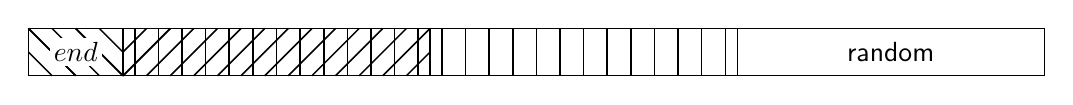
\begin{tikzpicture}
        \def\one{0.6}
        \def\scale{0.9}
        \def\nodeWidth{1.95}
        \def\endWidth{1.2}
        \def\width{3*2*\nodeWidth+\endWidth}
        \foreach \i\name in{0/B,1/C,2/D,3/Z} {
                \ifnum\i=2
                    \def\a{7.8}
                    \def\diff{7.2}
                \fi

                \ifnum\i=1
                    \def\a{3.9}
                    \def\diff{3.3}
                \fi

                \ifnum\i=0
                    \def\a{\endWidth}
                    \def\diff{0.6}
                \fi


                \def\b{0.6}
                \def\lw{0.2}

                \ifnum\i=0
                    \foreach \x [count=\i] in{0,0.3,0.6,...,\b}{
                            \draw [line width=\lw mm](\x,0)--(0,\x) (\a-\b+\x,\b)--(\a,\x);
                        }
                    \foreach \x [count=\i] in{0,0.3,0.6,...,\diff}{
                            \draw [line width=\lw mm](\x+\b,0)--(\x,\b);
                        }

                \fi
                \begin{scope}[shift={(\endWidth,0)}]
                    \ifnum\i=1
                        \foreach \x [count=\i] in{0,0.3,0.6,...,\b}{
                                \draw [line width=\lw mm](0,\x)--(\b-\x,\b) (\a-\b+\x,0)--(\a,\b-\x);
                            }
                        \foreach \x [count=\i] in{0,0.3,0.6,...,\diff}{
                                \draw [line width=\lw mm](\x,0)--(\b+\x,\b);
                            }
                    \fi

                    \ifnum\i=2
                        \foreach \x [count=\i] in{0.15,0.45,...,\a}{
                                \draw [line width=\lw mm](\x,0)--(\x,\b);
                            }
                    \fi
                \end{scope}

                \ifnum\i=3
                    \draw (\i*2*\nodeWidth-2*\nodeWidth+\endWidth,0) rectangle (\i*2*\nodeWidth+\endWidth,\one) node [midway] {\textsf{random}};
                \else
                    \ifnum\i>0
                        \draw (\i*2*\nodeWidth+\endWidth,0) -- (\i*2*\nodeWidth+\endWidth,\one);
                    \else
                        \draw [color=white] (\i*2*\nodeWidth,0) rectangle (\i*2*\nodeWidth+\endWidth,\one) node [midway,color=black,fill=white,inner sep=1.5pt] {$end$};
                        \draw (\endWidth,0) -- (\endWidth,\one);
                    \fi
                \fi
            }

        \draw (0,0) rectangle (\width,\one);
        % \draw[decoration={brace,raise=5pt},decorate] (\endWidth,\one) -- node[above=5pt] {filler string } (\width,\one);
        % \draw[decoration={brace,mirror,raise=5pt},decorate] (0,0) -- node[below=7pt] {Used for integrity check by $Z$} (\width,0);

    \end{tikzpicture}
    \caption{tbd}
\end{figure}